\documentclass[a4paper,11pt,notitlepage]{article}
\usepackage{amsmath}
\usepackage{amsfonts}
\usepackage{amssymb}
\usepackage[UTF8]{ctex}
\usepackage{graphicx}
\usepackage{color}
\usepackage{changepage}
\usepackage{enumitem}
\usepackage{subfigure}
\usepackage{float}
\usepackage[backend=biber]{biblatex}

\usepackage{titlesec}
\titleformat{\section}{\bfseries\Large}{$\S$\,\thesection}{1em}{}
\titleformat{\subsection}{\bfseries\large}{\Roman{subsection}}{1em}{}
\titleformat{\subsubsection}{\bfseries\normalsize}{\roman{subsubsection}}{1em}{}
\titlespacing*{\subsection}{2em}{2pt}{2pt}
\titlespacing*{\subsubsection}{3em}{2pt}{2pt}
\title{\vspace{-1.5cm} \textbf{\huge{数值分析期末上机}}\vspace{-1em}}
\author{By 211870125 陈睿硕}
\date{}

\usepackage{geometry}
\geometry{left=2cm,right=2cm,top=2cm,bottom=2cm}

\usepackage{fancyhdr}
\pagestyle{fancy}
\fancyhf{}
\fancyhead[L]{Final exam}
\fancyhead[R]{\thepage}
\setlength{\headheight}{14pt}

\definecolor{darkgreen}{RGB}{0,150,0}

\usepackage{listings}  % 引入 listings 包
\lstset{                % 定义代码块的样式
    basicstyle=\normalsize\ttfamily, % 设定代码字体大小、样式
    showspaces=false,   % 不显示空格
    showstringspaces=false, % 不显示字符串中的空格
    showtabs=false,     % 不显示制表符
    frame=single,       % 设定代码块边框样式
    rulecolor=\color{black}, % 设定代码块边框颜色
    tabsize=4,          % 设定制表符长度为 4 个字符
    captionpos=t,       % 设定标题位置为底部
    keywordstyle=\bfseries\color{blue}\ttfamily,
    stringstyle=\color{red}\ttfamily,
    commentstyle=\color{darkgreen}\ttfamily,
    morecomment=[l][\color{magenta}]{\#},
    framesep=0.5em,
    frameround=tttt,
    breaklines=true,    % 自动换行
    breakatwhitespace=false, % 只在空格分割处换行
    escapeinside={\%*}{*)}   % 允许使用 LaTeX 命令
}
\renewcommand{\lstlistingname}{代码}

\usepackage{hyperref}
\usepackage{cleveref}
\crefname{theorem}{定理}{定理}
\crefname{figure}{图}{图}
\crefname{equation}{式}{式}
\crefname{listing}{代码}{代码}
\crefname{table}{表}{表}

\begin{document}
\maketitle
\vspace{-1cm}
\thispagestyle{fancy}

\section{问题}
\begin{adjustwidth}{1em}{0pt}
\begin{enumerate}[label=\textbf{Q\arabic*}]
    \item 
    应用经典的四阶Runge-Kutta方法数值求解如下问题
    \[    
    \begin{cases}
            y''+\frac{2}{x}y'-\frac{6}{x^2}y=5-6x+7x^2,1<x<2\\
            y(1)=\frac{1}{2},y(2)=4+4\ln 2 
    \end{cases}
    \]
该问题的真解为$y=x^2-x^3+\frac{1}{2}x^4+x^2\ln x$。\\
分别取步长$h=\frac{1}{200},\frac{1}{100},\frac{1}{50},\frac{1}{25},\frac{1}{10},
    \frac{1}{5},\frac{1}{4}$进行计算,根据数值结果给出误差收敛阶,对计算结果进行分析。\label{Q1}\notag
\end{enumerate}
\end{adjustwidth}

\section{算法思路}
\subsection{算法:经典的四阶Runge-Kutta方法}
即4级四阶Runge-Kutta方法:
\[
\begin{cases}
        y_{n+1}=y_n+\frac{h}{6}(K_1+2K_2+2K_3+K_4)\\
        K_1=f(x_n,y_n)\\
        K_2=f(x_n+\frac{1}{2}h,y_n+\frac{1}{2}hK_1)\\
        K_3=f(x_n+\frac{1}{2}h,y_n+\frac{1}{2}hK_2)\\
        K_4=f(x_n+h,y_n+hK_3)
\end{cases}
\]
\subsection{对\ref{Q1}的解答}
事实上,对于这个问题,我们也可以使用高阶微分方程的四阶Runge-Kutta方法,但是我们这里发现,我们可以将题目式子化简为
\[    
    \begin{cases}
            (y'+\frac{3}{x}y)'=\frac{1}{x}(y'+\frac{3}{x}y)+5-6x+7x^2,1<x<2\\
            y(1)=\frac{1}{2},y(2)=4+4\ln 2
    \end{cases}
\]
进而使用常微分方程方法,可以进一步化简为
\[\begin{cases}
    y'=-\frac{3}{x}y+6x-6x^2+\frac{7}{2}x^3+5x\ln x,1<x<2\\
    y(1)=\frac{1}{2},y(2)=4+4\ln 2
\end{cases}\]
\indent 于是我们可以直接令四阶经典Runge-Kutta方法中的$f(x,y)=-\frac{3}{x}y+6x-6x^2+\frac{7}{2}x^3+5x\ln x$。
使用python实现算法,见\cref{code1.1}。计算出在x=2处经典的四阶Runge-Kutta方法
的误差(绝对值)和h的关系如\cref{pic:1}。
\begin{figure}[H]
    \centering
    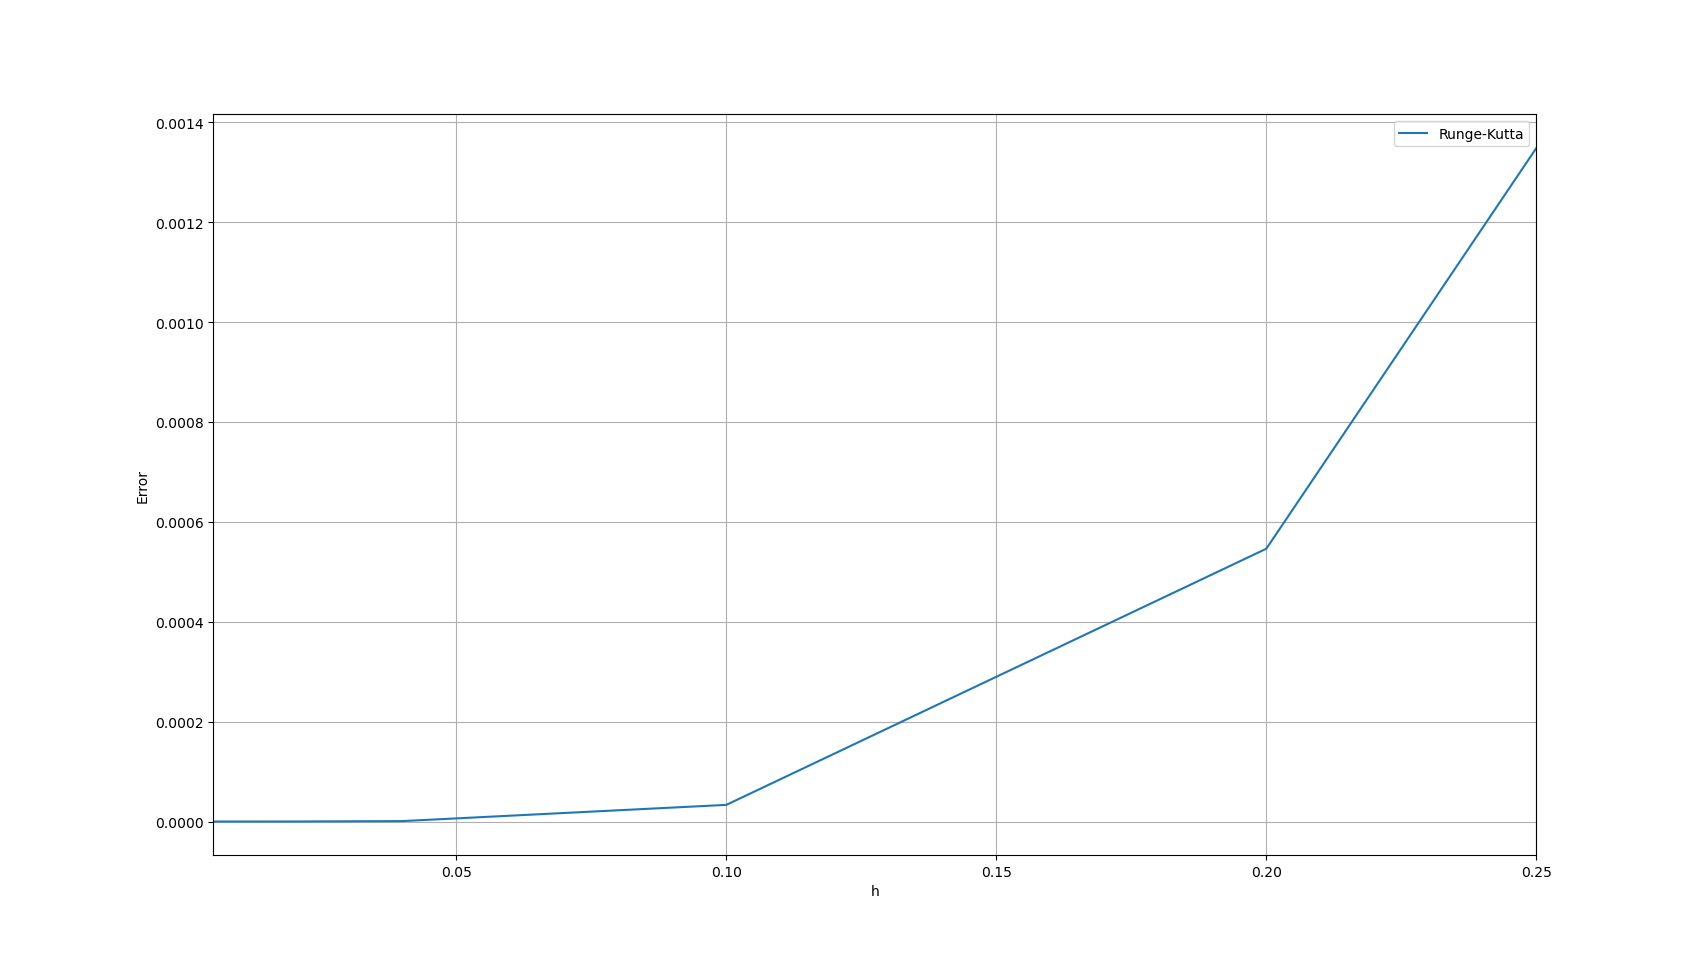
\includegraphics[width=0.8\textwidth]{../picture/Final exam.png}
    \caption{x=2处误差(绝对值)和h的关系}
    \label{pic:1}
\end{figure}
得到x=2处的误差与h值的对应如\cref{tab:1}。
\begin{table}[ht]
    \begin{center}
    \begin{tabular}{|c|c|}
        \hline
        h & Error(x=2) \\
        \hline
        0.005 & 2.02958539e-10 \\
        \hline
        0.01 & 3.25197380e-09 \\
        \hline
        0.02 & 5.21786614e-08 \\
        \hline
        0.04 & 8.39503355e-07 \\
        \hline
        0.1 & 3.33185076e-05\\
        \hline
        0.2& 5.46120318e-04\\
        \hline
        0.25&1.34812243e-03\\
        \hline
        \end{tabular}
        \caption{x=2处的误差}
        \label{tab:1}
    \end{center}
\end{table}
\\ \indent 为了分析其误差收敛阶,我们对h与x=2处的误差两者的对数做线性拟合,拟合结果为$\ln error = 4.0152541352629365\ln h + -1.0543858312344068$,
如\cref{pic:2},使用python的实现见\cref{code1.2}。
\begin{figure}[H]
    \centering
    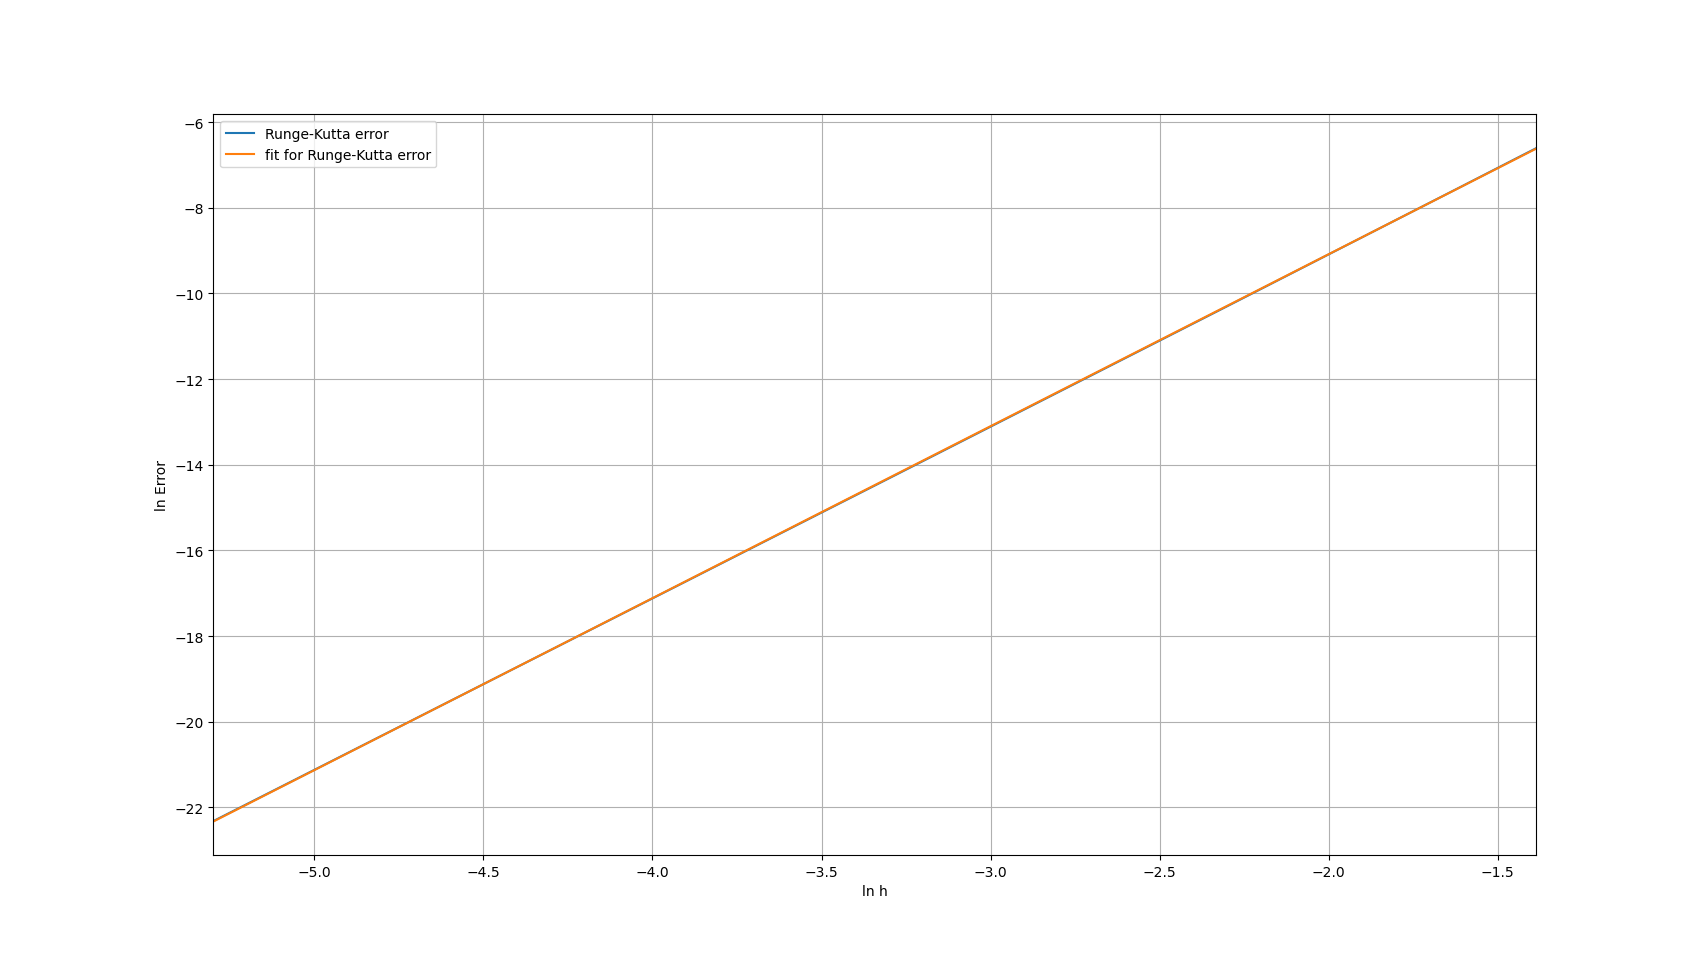
\includegraphics[width=0.8\textwidth]{../picture/Final exam extra.png}
    \caption{误差(绝对值)对数和h对数的拟合}
    \label{pic:2}
\end{figure}
\section{结果分析}
\subsection{对\ref{Q1}的分析}
可以看到,\cref{pic:2}中拟合程度较高,所以我们基本可以判断这个方法的误差收敛阶应该为4。事实上,这个结果也与我们
理论学习中得到的结论相符合。
\section{附录:程序代码}
\begin{lstlisting}[language=Python,caption={Final exam1.py},label={code1.1}]
import numpy as np
from matplotlib import pyplot as plt

def y(x):
    return x**2-x**3+1/2*x**4+x**2*np.log(x)

def f(x, y):
    return (-3/x)*y+6*x-6*x**2+7/2*x**3+5*x*np.log(x)


def runge_kutta(x, y0, f):
    y = np.zeros(x.shape)
    y[0] = y0
    for i in range(len(x) - 1):
        k1 = f(x[i], y[i])
        k2 = f(x[i] + h/2, y[i] + h/2 * k1)
        k3 = f(x[i] + h/2, y[i] + h/2 * k2)
        k4 = f(x[i] + h, y[i] + h * k3)
        y[i+1] = y[i] + h * (k1 + 2*k2 + 2*k3 + k4) / 6
    return y

h_list = [1/200,1/100,1/50,1/25,1/10,1/5,1/4]
error_x_eq_2=np.zeros(len(h_list))
y0 = 1/2
for i in range(len(h_list)):
    h=h_list[i]
    n=int(1/h)
    x = np.linspace(1, 2, n+1)
    y_cal=runge_kutta(x, y0, f)
    error_x_eq_2[i]=np.abs(y_cal[-1]-y(2))
print(error_x_eq_2)

plt.figure(figsize=(12, 8))
plt.plot(h_list, error_x_eq_2, label='Runge-Kutta')
plt.legend(loc='best')
plt.xlabel('h')
plt.ylabel('Error')
plt.xlim((1/200,1/4))
plt.grid(True)
plt.show()       
\end{lstlisting}

\begin{lstlisting}[language=Python,caption={Final exam2.py},label={code1.2}]
import numpy as np
from matplotlib import pyplot as plt

def y(x):
    return x**2-x**3+1/2*x**4+x**2*np.log(x)

def f(x, y):
    return (-3/x)*y+6*x-6*x**2+7/2*x**3+5*x*np.log(x)


def runge_kutta(x, y0, f):
    y = np.zeros(x.shape)
    y[0] = y0
    for i in range(len(x) - 1):
        k1 = f(x[i], y[i])
        k2 = f(x[i] + h/2, y[i] + h/2 * k1)
        k3 = f(x[i] + h/2, y[i] + h/2 * k2)
        k4 = f(x[i] + h, y[i] + h * k3)
        y[i+1] = y[i] + h * (k1 + 2*k2 + 2*k3 + k4) / 6
    return y

h_list = [1/200,1/100,1/50,1/25,1/10,1/5,1/4]
error_x_eq_2=np.zeros(len(h_list))
y0 = 1/2
for i in range(len(h_list)):
    h=h_list[i]
    n=int(1/h)
    x = np.linspace(1, 2, n+1)
    y_cal=runge_kutta(x, y0, f)
    error_x_eq_2[i]=np.abs(y_cal[-1]-y(2))
print(error_x_eq_2)

h_list_log=np.log(h_list)
error_x_eq_2_log=np.log(error_x_eq_2)

coefficients = np.polyfit(
    h_list_log, error_x_eq_2_log, 1)
print(
    f"对于拟合的函数式为 ln(error) = {coefficients[0]}ln(h) + {coefficients[1]}")
error_log_fit=coefficients[0]*h_list_log+coefficients[1]

plt.figure(figsize=(12, 8))
plt.plot(h_list_log, error_x_eq_2_log, label='Runge-Kutta error')
plt.plot(h_list_log, error_log_fit, label='fit for Runge-Kutta error')
plt.legend(loc='best')
plt.xlabel('ln h')
plt.ylabel('ln Error')
plt.xlim((np.log(1/200),np.log(1/4)))
plt.grid(True)
plt.show()       
\end{lstlisting}
\end{document}